\documentclass{beamer}
\usepackage[utf8]{inputenc}
\usepackage{tikz}
\usetikzlibrary{arrows,matrix,positioning,quotes}

\title{Barbed Bisimulations}
\author{Martin \textsc{Vassor}}
\institute{EPFL}
\beamertemplatenavigationsymbolsempty
\setbeamertemplate{footline}[frame number]

\begin{document}

\begin{frame}
	\titlepage
\end{frame}

\begin{frame}
	\frametitle{Introduction}
	\begin{itemize}
		\item Milner and Sangiorgi, $1980 \sim 1990$.
		\item How to compare modules ?
		\item Originally developed for CCS (process calculi).
	\end{itemize}
\end{frame}

\begin{frame}
	\frametitle{Recap \& Notations}
	Relation: 
	\begin{itemize}
		\item $\mathcal{R} \subseteq A\times B$
		\item Set of pairs $\langle a, b\rangle$
	\end{itemize}

	Transition system: 
	\begin{itemize}
		\item Transition semantics: $\longrightarrow: S\times S$
		\item Describes the evolution of states of a system.
	\end{itemize}
\end{frame}

\begin{frame}[fragile]
	\frametitle{String barbed simulation}
	Relation $\mathcal{R}$ over two languages such that:
	\begin{itemize}
		\item preserves transition
		\item preserves observable behaviour
	\end{itemize}


	\begin{minipage}{.46\linewidth}
		\begin{tikzpicture}[text height = 2.0ex]
			\matrix (m) [matrix of math nodes, column sep = 7em, row sep = 7em]
			{
				\node (N1) {S_1}; & \node (N2) {S_2};\\
				\node (N3) {\mathcal{R}(S_1)}; & \node (N4) {\mathcal{R}(S_2)};\\
			};

			\path (N1) edge[->] node [right] {$\mathcal{R}$} (N3);
			\path (N1) edge[->] node [above] {$\longrightarrow$} (N2);
			\path (N3) edge[->] node [above] {$\longrightarrow$} (N4);
			\path (N2) edge[->] node [right] {$\mathcal{R}$} (N4);

		\end{tikzpicture}
	\end{minipage}
	\hspace*{\fill}
	\begin{minipage}{.46\linewidth}
		\begin{flushright}
			$S\downarrow \Rightarrow \mathcal{R}(S)\downarrow$
		\end{flushright}
	\end{minipage}

\end{frame}

\begin{frame}
	\frametitle{Example: strong barbed (bi)simulation}
	\begin{minipage}{.46\linewidth}
		Transition:\\
		\begin{center}
			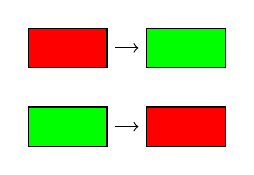
\begin{tikzpicture}[text height = 2.0ex]
				\draw[fill=red] (0, 1) rectangle (1, 1.5);
				\draw[fill=green] (1.5, 1) rectangle (2.5, 1.5);
				\draw[->]  (1.1, 1.25) to (1.4, 1.25);

				\draw[fill=green] (0, 0) rectangle (1, 0.5);
				\draw[fill=red] (1.5, 0) rectangle (2.5, 0.5);
				\draw[->]  (1.1, 0.25) to (1.4, 0.25);
			\end{tikzpicture}
		\end{center}

		Observable:\\
		\begin{center}
			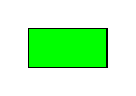
\begin{tikzpicture}[text height = 2.0ex]
				\draw[fill=green] (1.5, 1) rectangle (2.5, 1.5);
			\end{tikzpicture}
		\end{center}
	\end{minipage}
	\hspace*{\fill}
	\begin{minipage}{.46\linewidth}
		Transition:\\
		\begin{center}
			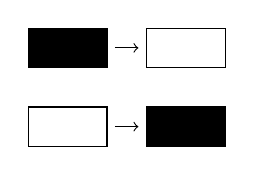
\begin{tikzpicture}[text height = 2.0ex]
				\draw[fill=black] (0, 1) rectangle (1, 1.5);
				\draw[fill=white] (1.5, 1) rectangle (2.5, 1.5);
				\draw[->]  (1.1, 1.25) to (1.4, 1.25);

				\draw[fill=white] (0, 0) rectangle (1, 0.5);
				\draw[fill=black] (1.5, 0) rectangle (2.5, 0.5);
				\draw[->]  (1.1, 0.25) to (1.4, 0.25);
			\end{tikzpicture}
		\end{center}
		Observable:\\
		\begin{center}
			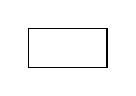
\begin{tikzpicture}[text height = 2.0ex]
				\draw[fill=white] (1.5, 1) rectangle (2.5, 1.5);
			\end{tikzpicture}
		\end{center}
	\end{minipage}

	\vspace*{\fill}

	$\mathcal{R} = \{\langle$
			
\begin{tikzpicture}
				\draw[fill=red] (0, 0) rectangle (1, 0.4);
			\end{tikzpicture} $, $
			
\begin{tikzpicture}
				\draw[fill=black] (0, 0) rectangle (1, 0.4);
			\end{tikzpicture}
		$\rangle;\langle$
			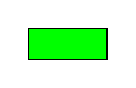
\begin{tikzpicture}
				\draw[fill=green] (0, 0) rectangle (1, 0.4);
			\end{tikzpicture} $, $
			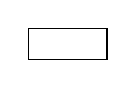
\begin{tikzpicture}
				\draw[fill=white] (0, 0) rectangle (1, 0.4);
			\end{tikzpicture}
		$\rangle\}$
\end{frame}


\begin{frame}
	\frametitle{Extensions}
	\begin{itemize}
		\item Bisimulation: $\mathcal{R}$ and $\mathcal{R}^{-1}$ are simulations.
		\item Weak form: No ``one-to-one'' transition mapping.
	\end{itemize}
\end{frame}

\begin{frame}
	\frametitle{Conclusion}
	\begin{itemize}
		\item Defining ``observable''
		\item Internal behaviour vs. Observable
		\item Widely used in process calculi
	\end{itemize}
\end{frame}

\begin{frame}
	\frametitle{References}
	\nocite{*}
	\bibliographystyle{plain}
	\bibliography{ref} 
\end{frame}

\end{document}
